% Title: gl2ps_renderer figure
% Creator: GL2PS 1.4.0, (C) 1999-2017 C. Geuzaine
% For: Octave
% CreationDate: Sun Dec  1 20:36:38 2019
\setlength{\unitlength}{1pt}
\begin{picture}(0,0)
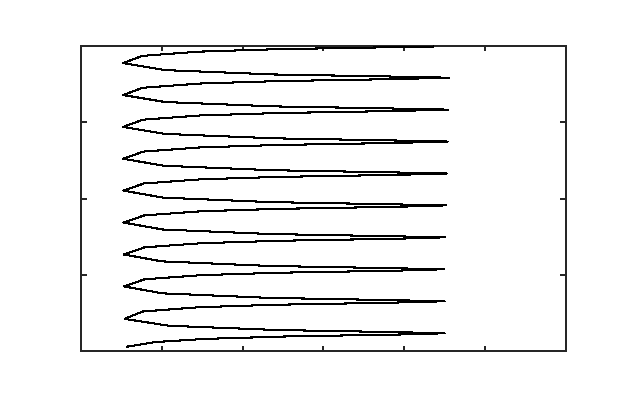
\includegraphics{img/phaseThetaPhi-inc}
\end{picture}%
\begin{picture}(300,200)(0,0)
\fontsize{10}{0}
\selectfont\put(39,24){\makebox(0,0)[t]{\textcolor[rgb]{0.15,0.15,0.15}{{0.2}}}}
\fontsize{10}{0}
\selectfont\put(77.75,24){\makebox(0,0)[t]{\textcolor[rgb]{0.15,0.15,0.15}{{0.4}}}}
\fontsize{10}{0}
\selectfont\put(116.5,24){\makebox(0,0)[t]{\textcolor[rgb]{0.15,0.15,0.15}{{0.6}}}}
\fontsize{10}{0}
\selectfont\put(155.25,24){\makebox(0,0)[t]{\textcolor[rgb]{0.15,0.15,0.15}{{0.8}}}}
\fontsize{10}{0}
\selectfont\put(194,24){\makebox(0,0)[t]{\textcolor[rgb]{0.15,0.15,0.15}{{1}}}}
\fontsize{10}{0}
\selectfont\put(232.75,24){\makebox(0,0)[t]{\textcolor[rgb]{0.15,0.15,0.15}{{1.2}}}}
\fontsize{10}{0}
\selectfont\put(271.5,24){\makebox(0,0)[t]{\textcolor[rgb]{0.15,0.15,0.15}{{1.4}}}}
\fontsize{10}{0}
\selectfont\put(34.0107,31.4757){\makebox(0,0)[r]{\textcolor[rgb]{0.15,0.15,0.15}{{0}}}}
\fontsize{10}{0}
\selectfont\put(34.0107,68.1068){\makebox(0,0)[r]{\textcolor[rgb]{0.15,0.15,0.15}{{10}}}}
\fontsize{10}{0}
\selectfont\put(34.0107,104.738){\makebox(0,0)[r]{\textcolor[rgb]{0.15,0.15,0.15}{{20}}}}
\fontsize{10}{0}
\selectfont\put(34.0107,141.369){\makebox(0,0)[r]{\textcolor[rgb]{0.15,0.15,0.15}{{30}}}}
\fontsize{10}{0}
\selectfont\put(34.0107,178){\makebox(0,0)[r]{\textcolor[rgb]{0.15,0.15,0.15}{{40}}}}
\fontsize{11}{0}
\selectfont\put(155.25,11){\makebox(0,0)[t]{\textcolor[rgb]{0.15,0.15,0.15}{{$\theta$}}}}
\fontsize{11}{0}
\selectfont\put(17.0107,104.738){\rotatebox{90}{\makebox(0,0)[b]{\textcolor[rgb]{0.15,0.15,0.15}{{$\phi$}}}}}
\fontsize{11}{0}
\selectfont\put(155.25,188){\makebox(0,0)[b]{\textcolor[rgb]{0,0,0}{{Diagrama fase de $\theta - \phi$}}}}
\end{picture}
